%%%%%%%%%%%%%%%%%%%%%%%%%%%%%%%%%%%%%%%%%%%%%%%%%%%
%% LaTeX book template                           %%
%% Author:  Amber Jain (http://amberj.devio.us/) %%
%% License: ISC license                          %%
%%%%%%%%%%%%%%%%%%%%%%%%%%%%%%%%%%%%%%%%%%%%%%%%%%%

\documentclass[a4paper,11pt,oneside]{book}
\usepackage{modulestyle}

%%%%%%%%%%%%%%%%%%%%%%%%%%%%%%%%%%%%%%%%%%%%%%%%%%%%%%%%%
% Source: http://en.wikibooks.org/wiki/LaTeX/Hyperlinks %
%%%%%%%%%%%%%%%%%%%%%%%%%%%%%%%%%%%%%%%%%%%%%%%%%%%%%%%%%

%%%%%%%%%%%%%%%%%%%%%%%%%%%%%%%%%%%%%%%%%%%%%%%%%%%%%%%%%%%%%%%%%%%%%%%%%%%%%%%%
% 'dedication' environment: To add a dedication paragraph at the start of book %
% Source: http://www.tug.org/pipermail/texhax/2010-June/015184.html            %
%%%%%%%%%%%%%%%%%%%%%%%%%%%%%%%%%%%%%%%%%%%%%%%%%%%%%%%%%%%%%%%%%%%%%%%%%%%%%%%%
\newenvironment{dedication}
{
   \cleardoublepage
   \thispagestyle{empty}
   \vspace*{\stretch{1}}
   \hfill\begin{minipage}[t]{0.66\textwidth}
   \raggedright
}
{
   \end{minipage}
   \vspace*{\stretch{3}}
   \clearpage
}

%%%%%%%%%%%%%%%%%%%%%%%%%%%%%%%%%%%%%%%%%%%%%%%%
% Chapter quote at the start of chapter        %
% Source: http://tex.stackexchange.com/a/53380 %
%%%%%%%%%%%%%%%%%%%%%%%%%%%%%%%%%%%%%%%%%%%%%%%%
\makeatletter
\renewcommand{\@chapapp}{}% Not necessary...
\newenvironment{chapquote}[2][2em]
  {\setlength{\@tempdima}{#1}%
   \def\chapquote@author{#2}%
   \parshape 1 \@tempdima \dimexpr\textwidth-2\@tempdima\relax%
   \itshape}
  {\par\normalfont\hfill--\ \chapquote@author\hspace*{\@tempdima}\par\bigskip}
\makeatother

%%%%%%%%%%%%%%%%%%%%%%%%%%%%%%%%%%%%%%%%%%%%%%%%%%%
% First page of book which contains 'stuff' like: %
%  - Book title, subtitle                         %
%  - Book author name                             %
%%%%%%%%%%%%%%%%%%%%%%%%%%%%%%%%%%%%%%%%%%%%%%%%%%%

\newcommand{\BookTitle}{Applications Development and Emerging Technologies}
\newcommand{\BookTitleFootnote}{A course in the Bachelor of Science in Computer Science.}

\newcommand{\BookSubtitle}{A Study Guide for Students of Sorsogon State University - Bulan Campus}
\newcommand{\BookSubtitleFootnote}{This book is a study guide for students of
Sorsogon State University - Bulan Campus taking up the course Applications Development and Emerging Technologies.}

\newcommand{\BookAuthorFirstName}{Jarrian Vince}
\newcommand{\BookAuthorLastName}{Gojar}
\newcommand{\BookAuthorName}{Jarrian Vince G. Gojar}
\newcommand{\BookAuthorURL}{https://github.com/godkingjay}

% Book's title and subtitle
\title{\Huge \textbf{\BookTitle}  \footnote{\BookTitleFootnote} \\
\huge \BookSubtitle \footnote{\BookSubtitleFootnote}}

% Author
\author{\textsc{\BookAuthorName}\thanks{\url{\BookAuthorURL}}}

\begin{document}

\frontmatter
\maketitle

%%%%%%%%%%%%%%%%%%%%%%%%%%%%%%%%%%%%%%%%%%%%%%%%%%%%%%%%%%%%%%%
% Add a dedication paragraph to dedicate your book to someone %
%%%%%%%%%%%%%%%%%%%%%%%%%%%%%%%%%%%%%%%%%%%%%%%%%%%%%%%%%%%%%%%
\begin{dedication}
  Sorsogon State University - Bulan Campus
\end{dedication}

%%%%%%%%%%%%%%%%%%%%%%%%%%%%%%%%%%%%%%%%%%%%%%%%%%%%%%%%%%%%%%%%%%%%%%%%
% Auto-generated table of contents, list of figures and list of tables %
%%%%%%%%%%%%%%%%%%%%%%%%%%%%%%%%%%%%%%%%%%%%%%%%%%%%%%%%%%%%%%%%%%%%%%%%
\tableofcontents
\listoffigures
\listoftables
\lstlistoflistings

\mainmatter

%%%%%%%%%%%
% Preface %
%%%%%%%%%%%
\chapter*{Preface}
% A Quote all about Applications Development and Emerging Technologies
\begin{chapquote}{}
\end{chapquote}

\noindent \BookAuthorName \\
\noindent \url{\BookAuthorURL}

%%%%%%%%%%%%%%%%%%%%%%%%%%%%%%%%%%%%
%%%%%~ NEW CHAPTER STARTS HERE %%%%%
%%%%%%%%%%%%%%%%%%%%%%%%%%%%%%%%%%%%
\chapter{Introduction to Applications Development and Emerging Technologies}

\section{Introduction}

\subsection{Application}

An \textbf{application} is a software program that allows users to perform
specific tasks. Applications for desktop or laptop computers are sometimes
called \textbf{desktop applications}, while those for mobile devices are called
\textbf{mobile apps}. When you open an application, it runs inside the
operating system until you close it. Most of the time, you will have more than
one application open at the same time, which is known as \textbf{multitasking}.

\subsection{Development}

\textbf{Development} is the process of creating a software application.
It includes designing the user interface, writing code, and testing
the application for bugs. The goal of software development is to
create a program that is easy to use and works correctly.

\subsection{Application Development}

\textbf{Application development} is the process of planning, designing,
creating, testing, and deploying an application to perform various
business operations. It can be done by massive organizations with large
teams working on projects or by a single freelance developer.

% \section{Software Development Life Cycle}

% The \textbf{software development life cycle} (SDLC) is a process used by
% software developers to design, develop, and test software applications.
% The SDLC consists of several phases, including planning, analysis, design,
% implementation, and maintenance.

% \subsection{Different Types of Software Development Life Cycle Models}

% There are several different types of software development life cycle models,
% including:

% \begin{itemize}
%   \item Waterfall Model
%   \item Agile Model
%   \item Spiral Model
%   \item V-Model
%   \item Iterative Model
% \end{itemize}

% \subsubsection{Waterfall Model}

% The \textbf{waterfall model} is a linear and sequential approach to software
% development. It consists of several phases, including requirements gathering,
% analysis, design, coding/implementation, testing, and maintenance. Each phase
% must be completed before moving on to the next phase.

% % Image from ./assets/sdlc/waterfall.png
% \begin{figure}[H]
%   \centering
%   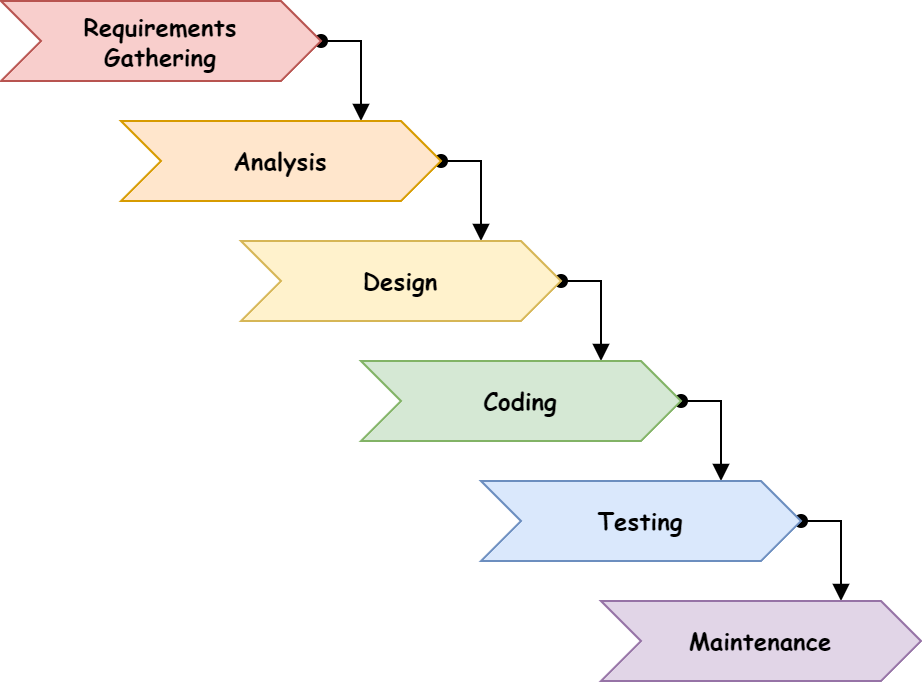
\includegraphics[width=1\textwidth]{./assets/sdlc/waterfall.png}
%   \caption{Waterfall Model}
%   \label{fig:waterfall}
% \end{figure}

% Figure \ref{fig:waterfall} shows the waterfall model.

% \begin{itemize}
%   \item \textbf{Requirements Gathering:} In this phase, the requirements
%   for the software application are gathered from the client or end-users.
%   This phase answers the question, "What does the customer want?".

%   \item \textbf{Analysis:} In this phase, the requirements gathered in the
%   previous phase are analyzed to determine the feasibility of the project.
%   This phase answers the question, "What is the best way to achieve the
%   customer's requirements?".

%   \item \textbf{Design:} In this phase, the software application is
%   designed based on the requirements gathered in the previous phases.
%   This phase answers the question, "How will the software application
%   look and function?".

%   \item \textbf{Coding/Implementation:} In this phase, the software
%   application is developed based on the design created in the previous
%   phase. This phase answers the question, "How will the software
%   application be built?".

%   \item \textbf{Testing:} In this phase, the software application is
%   tested to ensure that it works correctly and meets the requirements
%   specified by the client or end-users. This phase answers the question,
%   "Does the software application work as expected?".

%   \item \textbf{Maintenance:} In this phase, the software application is
%   maintained and updated to fix any bugs or issues that arise after the
%   application has been deployed. This phase answers the question, "How
%   can the software application be improved?".
% \end{itemize}

% \subsubsection{Agile Model}

% The \textbf{agile model} is an iterative and incremental approach to
% software development. It consists of several phases, including planning,
% design, coding, testing, and deployment. The agile model allows for
% flexibility and adaptability throughout the development process.

% % Image from ./assets/sdlc/agile.png

\section{Different Types of Application Development}

There are several different types of application development, including:

\begin{itemize}
  \item Web Development
  \item Mobile Application Development
  \item Desktop Application Development
  \item Game Development
  \item Cloud Development
\end{itemize}

\subsection{Web Development}

\textbf{Web development} is the process of creating websites and web
applications. It involves designing the user interface, writing code,
and testing the website for bugs. Web development can be divided into
two categories: front-end development and back-end development.

\subsubsection{Front-End Development}

\textbf{Front-end development} is the process of creating the user
interface of a website. It involves designing the layout, colors, and
fonts of the website. Front-end developers use HTML, CSS, and JavaScript
to create the user interface of a website.

\begin{enumerate}
  \item \textbf{HTML (HyperText Markup Language)} is the standard markup
        language used to create web pages. It defines the structure of a web
        page using a series of elements.

  \item \textbf{CSS (Cascading Style Sheets)} is a style sheet language
        used to define the appearance of a web page. It allows developers to
        control the layout, colors, and fonts of a website.

  \item \textbf{JavaScript} is a programming language used to create
        interactive elements on a web page. It allows developers to add
        functionality such as animations, pop-ups, and form validation to a
        website.

  \item \textbf{Bootstrap} is a front-end framework that allows developers
        to create responsive and mobile-first websites. It provides a set of
        pre-designed components, such as buttons, forms, and navigation bars,
        that can be easily customized.

  \item \textbf{React} is a JavaScript library used to create user
        interfaces for single-page applications. It allows developers to build
        reusable components that update automatically when the data changes.

  \item \textbf{Angular} is a front-end framework that allows developers
        to create dynamic web applications. It provides a set of tools and
        libraries for building interactive user interfaces.

  \item \textbf{Vue} is a progressive JavaScript framework used to create
        user interfaces and single-page applications. It allows developers to
        build interactive web applications with ease.
\end{enumerate}

The above tools and technologies are commonly used in front-end development to
create responsive and interactive websites. HTML, CSS, and JavaScript are the
building blocks of front-end development, while frameworks such as Bootstrap,
React, Angular, and Vue provide additional features for building modern web
applications.

\subsubsection{Back-End Development}

\textbf{Back-end development} is the process of creating the server-side
logic of a website. It involves writing code that interacts with the
database and processes data. Back-end developers use programming languages
such as PHP, Python, and Ruby to create the server-side logic of a website.

\begin{enumerate}
  \item \textbf{Node.js} is a JavaScript runtime environment that allows
        developers to run JavaScript on the server-side. It provides a set of
        libraries and tools for building scalable and high-performance web
        applications.

  \item \textbf{Express} is a web application framework for Node.js. It
        provides a set of features for building web applications, such as routing,
        middleware, and templating.

  \item \textbf{Django} is a high-level web framework for Python. It allows
        developers to build web applications quickly and efficiently. Django
        provides a set of tools and libraries for building secure and scalable
        web applications.

  \item \textbf{Flask} is a lightweight web framework for Python. It allows
        developers to build web applications with minimal code. Flask provides
        a set of tools and libraries for building simple and scalable web
        applications.

  \item \textbf{Ruby on Rails} is a web application framework for Ruby. It
        provides a set of tools and libraries for building web applications
        quickly and efficiently. Ruby on Rails follows the convention over
        configuration principle, which allows developers to write less code
        and focus on building the application.

  \item \textbf{Laravel} is a web application framework for PHP. It
        provides a set of tools and libraries for building web applications
        quickly and efficiently. Laravel follows the model-view-controller
        (MVC) architecture, which allows developers to separate the business
        logic from the presentation layer.

  \item \textbf{Spring} is a web application framework for Java. It
        provides a set of tools and libraries for building enterprise-level
        web applications. Spring follows the inversion of control (IoC)
        principle, which allows developers to write loosely coupled code
        and focus on building the application.
\end{enumerate}

The above tools and technologies are commonly used in back-end development to
create the server-side logic of a website. Back-end developers use these tools
to interact with the database, process data, and handle user requests on the
server-side.

\subsection{Mobile Application Development}

\textbf{Mobile application development} is the process of creating mobile applications
for smartphones and tablets. It involves designing the user interface,
writing code, and testing the mobile application for bugs. Mobile
development can be divided into two categories: iOS development and
Android development.

\subsubsection{iOS Development}

\textbf{iOS development} is the process of creating mobile applications
for Apple devices, such as iPhones and iPads. It involves designing the
user interface using Xcode and writing code in Swift or Objective-C.
iOS developers use Xcode, Swift, and Objective-C to create mobile
applications for Apple devices.

\begin{enumerate}
  \item \textbf{Xcode} is an integrated development environment (IDE)
        used to create iOS applications. It provides a set of tools and
        libraries for building mobile applications for Apple devices.

  \item \textbf{Swift} is a programming language used to create iOS
        applications. It provides a set of features for building mobile
        applications, such as type safety, optionals, and generics.

  \item \textbf{Objective-C} is a programming language used to create
        iOS applications. It provides a set of features for building mobile
        applications, such as dynamic typing, message passing, and memory
        management.

  \item \textbf{React Native} is a JavaScript framework used to create
        mobile applications for Android and iOS devices. It allows developers
        to build cross-platform mobile applications with a single codebase.

  \item \textbf{Flutter} is a mobile UI framework used to create mobile
        applications for Android and iOS devices. It allows developers to build
        cross-platform mobile applications with a single codebase.
\end{enumerate}

The above tools and technologies are commonly used in iOS development to create
mobile applications for Apple devices. iOS developers use these tools to design
the user interface and write code for mobile applications.

\subsubsection{Android Development}

\textbf{Android development} is the process of creating mobile
applications for Android devices. It involves designing the user
interface using Android Studio and writing code in Java or Kotlin.
Android developers use Android Studio, Java, and Kotlin to create
mobile applications for Android devices.

\begin{enumerate}
  \item \textbf{Android Studio} is an integrated development environment
        (IDE) used to create Android applications. It provides a set of tools
        and libraries for building mobile applications for Android devices.

  \item \textbf{Java} is a programming language used to create Android
        applications. It provides a set of features for building mobile
        applications, such as object-oriented programming, inheritance, and
        polymorphism.

  \item \textbf{Kotlin} is a programming language used to create Android
        applications. It provides a set of features for building mobile
        applications, such as null safety, extension functions, and coroutines.

  \item \textbf{React Native} is a JavaScript framework used to create
        mobile applications for Android and iOS devices. It allows developers
        to build cross-platform mobile applications with a single codebase.

  \item \textbf{Flutter} is a mobile UI framework used to create mobile
        applications for Android and iOS devices. It allows developers to build
        cross-platform mobile applications with a single codebase.
\end{enumerate}

The above tools and technologies are commonly used in Android development to
create mobile applications for Android devices. Some of the tools here are also
used in iOS development to create mobile applications for Apple devices. React
Native and Flutter in particular are used to build cross-platform mobile
applications for both Android and iOS devices.

\subsection{Desktop Application Development}

\textbf{Desktop application development} is the process of creating desktop
applications for Windows, macOS, and Linux. It involves designing the
user interface, writing code, and testing the desktop application for
bugs.

\begin{enumerate}
  \item \textbf{Electron} is a framework used to create desktop
        applications with web technologies. It allows developers to build
        cross-platform desktop applications with HTML, CSS, and JavaScript.

  \item \textbf{JavaFX} is a framework used to create desktop applications
        with Java. It provides a set of tools and libraries for building
        cross-platform desktop applications with Java.

  \item \textbf{Qt} is a framework used to create desktop applications
        with C++. It provides a set of tools and libraries for building
        cross-platform desktop applications with C++.

  \item \textbf{WinForms} is a framework used to create desktop
        applications with C\#. It provides a set of tools and libraries for
        building desktop applications for Windows.

  \item \textbf{WPF} is a framework used to create desktop applications
        with C\#. It provides a set of tools and libraries for building
        desktop applications for Windows.
\end{enumerate}

The above tools and technologies are commonly used in desktop development to
create desktop applications for Windows, macOS, and Linux. For Windows,
developers use WinForms and WPF to create desktop applications with C\#. For
cross-platform desktop applications, developers use Electron, JavaFX, and Qt to
build desktop applications with web technologies, Java, and C++.

\subsection{Game Development}

\textbf{Game development} is the process of creating video games for
consoles, computers, and mobile devices. It involves designing the
gameplay, writing code, and testing the game for bugs.

\begin{enumerate}
  \item \textbf{Unity} is a game engine used to create 2D and 3D games
        for consoles, computers, and mobile devices. It provides a set of
        tools and libraries for building cross-platform games with C\#.

  \item \textbf{Unreal Engine} is a game engine used to create 2D and
        3D games for consoles, computers, and mobile devices. It provides a
        set of tools and libraries for building cross-platform games with C++.

  \item \textbf{Godot} is a game engine used to create 2D and 3D games
        for consoles, computers, and mobile devices. It provides a set of
        tools and libraries for building cross-platform games with GDScript.

  \item \textbf{GameMaker Studio} is a game engine used to create 2D
        games for consoles, computers, and mobile devices. It provides a set
        of tools and libraries for building cross-platform games with GML.

  \item \textbf{Construct} is a game engine used to create 2D games for
        consoles, computers, and mobile devices. It provides a set of tools
        and libraries for building cross-platform games with events.
\end{enumerate}

The above tools and technologies are commonly used in game development to
create video games for consoles, computers, and mobile devices. Unity, Unreal
Engine, Godot, GameMaker Studio, and Construct are popular game engines used by
game developers to create 2D and 3D games. These game engines provide a set of
tools and libraries for building cross-platform games with C\#, C++, GDScript,
and GML.

\subsection{Cloud Development}

\textbf{Cloud development} is the process of creating cloud-based
applications that run on remote servers. It involves designing the
user interface, writing code, and testing the cloud application for
bugs.

\begin{enumerate}
  \item \textbf{Amazon Web Services (AWS)} is a cloud platform used to
        create cloud-based applications. It was one of the first cloud
        platforms and is widely used by developers to build scalable and
        secure cloud applications. It is a subsidiary of Amazon providing
        on-demand cloud computing platforms and APIs to individuals,

  \item \textbf{Microsoft Azure}, similarly to AWS, is a cloud platform
        used to create cloud-based applications. Microsoft Azure is a cloud
        computing service created by Microsoft for building, testing, deploying,
        and managing applications and services through Microsoft-managed data
        centers.

  \item \textbf{Google Cloud Platform (GCP)}, similarly to AWS and
        Microsoft Azure, is a cloud platform used to create cloud-based
        applications. Google Cloud Platform is a suite of cloud computing
        services that runs on the same infrastructure that Google uses
        internally for its end-user products, such as Google Search, Gmail,
        file storage, and YouTube.

  \item \textbf{Heroku} is a cloud platform used to create cloud-based
        applications. It provides a set of tools and services for building
        scalable and secure cloud applications. Heroku is a cloud platform
        as a service supporting several programming languages.

  \item \textbf{Firebase}, also developed by Google, is a cloud
        platform used to create cloud-based applications. Firebase is a
        platform developed by Google for creating mobile and web applications.
        It was originally an independent company founded in 2011. In 2014,
        Google acquired the platform and it is now their flagship offering
        for app development.
\end{enumerate}

The above tools and technologies are commonly used in cloud development to
create cloud-based applications that run on remote servers. AWS, Microsoft
Azure, GCP, Heroku, and Firebase are popular cloud platforms used by developers
to build scalable and secure cloud applications. These cloud platforms provide
a set of tools and services for building cloud-based applications with ease.

\chapter{Web Development}

\section{Introduction}

There are around 3.58 billion internet users on the planet. This implies that
over half of the world's 7.6 billion people have access to the internet, which
they use for everything from entertainment to education, communication to
commerce, keeping up with current events, and keeping up with business experts.
Indeed, for most people, the internet is the first (and often only) channel
through which we communicate with the world in all of its complexities.

There are three interactive elements on the internet:

\begin{enumerate}
  \item \textbf{Websites} - A collection of web pages that are linked
        together and share a common domain name.

  \item \textbf{Servers} - A computer or computer program that manages
        access to a centralized resource or service in a network.

  \item \textbf{Browsers} - A software application used to access and
        view websites on the internet.
\end{enumerate}

The frontend (client side) and the backend (server side) are two parts of any
website. The frontend comprises everything the user sees and experiences
instantly while visiting a website. The backend is behind the scenes that
store, send and receive information.

HTML, CSS, and Javascript files make up everything a user sees on a website. As
a web developer, these are the most basic tools needed. They are the languages
that required to build websites.

\section{HTML}

\textbf{HTML (HyperText Markup Language)} is the standard markup language
used to create web pages. It defines the structure of a web page using a
series of elements. It contains the essential elements of a website, such
as words, titles, and paragraphs, as well as links, images, and other
media. HTML elements are represented by tags, which are enclosed in angle
brackets. HTML forms the backbone of any webpage, dictating its structure
and content.

\begin{lstlisting}[language=HTML, caption={HTML Example}, label={lst:html-example}]
<!DOCTYPE html>
<html lang="en">

<head>
    <meta charset="UTF-8" />
    <meta name="viewport" content="width=device-width, initial-scale=1.0" />
    <title>First Web Page</title>
</head>

<body>
    <h1>Hello, World!</h1>
    <p>Welcome to my website.</p>
</body>

</html>
\end{lstlisting}

Code \ref{lst:html-example} shows an example of an HTML document. An HTML
boilerplate usually looks like this:

\begin{itemize}
  \item \textbf{<!DOCTYPE html>} - Defines the document type and version
        of HTML. In this case, it is HTML5.
  \item \textbf{<html>} - Defines the root element of an HTML page.
  \item \textbf{<head>} - Contains meta-information about the document,
        such as the title, character set, and viewport.
  \item \textbf{<body>} - Contains the content of the document, such as
        headings, paragraphs, and images.
\end{itemize}

\subsection{HTML Tags}

HTML tags are used to define the structure and content of a web page. They are
enclosed in angle brackets and come in pairs: an opening tag and a closing tag.
The opening tag is used to define the beginning of an element, while the
closing tag is used to define the end of an element.

When an HTML tag is opened, it must be closed to avoid errors. Some tags are
self-closing, meaning they do not require a closing tag. HTML tags can also
have attributes, which provide additional information about the element.

% Example of Open and Close Tag
\begin{lstlisting}[language=HTML, caption={HTML Open and Close Tag}, label={lst:open-close-tag}]
<p>Welcome to my website.</p>
\end{lstlisting}

Code \ref{lst:open-close-tag} shows an example of an HTML tag with an opening
tag (\textbf{<p>}) and a closing tag (\textbf{</p>}). The content of the
paragraph is "Welcome to my website.".

% Example of Self-Closing Tag
\begin{lstlisting}[language=HTML, caption={HTML Self-Closing Tag}, label={lst:self-closing-tag}]
<img src="https://avatar.iran.liara.run/public" alt="Image" />
\end{lstlisting}

Code \ref{lst:self-closing-tag} shows an example of an HTML tag that is
self-closing (\textbf{<img />}). This tag is used to insert an image into the
document. The \textbf{src} attribute specifies the URL of the image, while the
\textbf{alt} attribute provides a text description of the image.

\subsubsection{<html>...</html>}

This tag specifies that the webpage is written in HTML. It appears at the very
first and last line of the webpage. It is mainly used to show that the page
uses HTML5 – the latest version of the language. Also known as the root
element, this tag can be thought of as a parent tag for every other tag used in
the page.

\begin{lstlisting}[language=HTML, caption={HTML <html> Tag}, label={lst:html-tag}]
<!DOCTYPE html>
<html lang="en">
    <!-- Content goes here -->
</html>
\end{lstlisting}

Code \ref{lst:html-tag} shows an example of the <html> tag. Here, the
\textbf{lang} attribute specifies the language of the document, which is
English in this case.

\subsubsection{<head>...</head>}

This tag is used to define the head section of the webpage. The head section
contains meta-information about the document, such as the title, character set,
and viewport. It is not displayed on the webpage but is used to provide
information about the document to the browser and search engines.

\begin{lstlisting}[language=HTML, caption={HTML <head> Tag}, label={lst:head-tag}]
<head>
    <meta charset="UTF-8" />
    <meta name="viewport" content="width=device-width, initial-scale=1.0" />
    <title>First Web Page</title>
</head>
\end{lstlisting}

Code \ref{lst:head-tag} shows an example of the <head> tag. Here, the
\textbf{<meta>} tag is used to define the character set and viewport of the
document, while the \textbf{<title>} tag is used to define the title of the
document. This title appears in the browser tab.

\subsubsection{<title>...</title>}

This tag is used to define the title of the document. It appears in the browser
tab and is used to identify the webpage.

\begin{lstlisting}[language=HTML, caption={HTML <title> Tag}, label={lst:title-tag}]
<title>First Web Page</title>
\end{lstlisting}

Code \ref{lst:title-tag} shows an example of the <title> tag. Here, the title
of the document is "First Web Page". This title appears in the browser tab when
the document is opened.

\subsubsection{<body>...</body>}

This tag is used to define the body section of the webpage. The body section
contains the content of the document, such as headings, paragraphs, and images.
It is displayed on the webpage and is visible to the user.

\begin{lstlisting}[language=HTML, caption={HTML <body> Tag}, label={lst:body-tag}]
<body>
    <h1>Hello, World!</h1>
    <p>Welcome to my website.</p>
</body>
\end{lstlisting}

Code \ref{lst:body-tag} shows an example of the <body> tag. Here, the
\textbf{<h1>} tag is used to define a heading, while the \textbf{<p>} tag is
used to define a paragraph. This content is displayed on the webpage and is
visible to the user.

\subsubsection{<h1>...</h1> to <h6>...</h6>}

These tags are used to define headings of different sizes. The \textbf{<h1>}
tag defines the largest heading, while the \textbf{<h6>} tag defines the
smallest heading. Headings are used to define the structure of the document and
provide a hierarchy of information.

\begin{lstlisting}[language=HTML, caption={HTML <h1> to <h6> Tags}, label={lst:h-tag}]
<h1>This is a Heading 1</h1>
<h2>This is a Heading 2</h2>
<h3>This is a Heading 3</h3>
<h4>This is a Heading 4</h4>
<h5>This is a Heading 5</h5>
<h6>This is a Heading 6</h6>
\end{lstlisting}

Code \ref{lst:h-tag} shows an example of the \textbf{<h1>} to \textbf{<h6>}
tags. These tags are used to define headings of different sizes, with
\textbf{<h1>} being the largest and \textbf{<h6>} being the smallest.

\subsubsection{<p>...</p>}

This tag is used to define a paragraph of text. It is used to group text
content together and provide structure to the document.

\begin{lstlisting}[language=HTML, caption={HTML <p> Tag}, label={lst:p-tag}]
<p>
  Excepteur officia tempor do laborum commodo cupidatat ea Lorem qui irure enim velit. Adipisicing dolor minim Lorem nulla dolor quis et aliqua. Officia anim adipisicing excepteur sint elit qui laboris reprehenderit non elit. Voluptate voluptate duis aliqua proident elit exercitation cillum anim reprehenderit nostrud minim culpa veniam.
</p>
\end{lstlisting}

Code \ref{lst:p-tag} shows an example of the \textbf{<p>} tag. This tag is used
to define a paragraph of text, which is displayed on the webpage.

\subsubsection{<div>...</div>}

This tag is used to define a division or section of the document. It is a
block-level element that can contain other block-level or inline elements.

\begin{lstlisting}[language=HTML, caption={HTML <div> Tag}, label={lst:div-tag}]
<div>
    <h1>Hello, World!</h1>
    <p>Welcome to my website.</p>
</div>

<div>
    <img src="https://avatar.iran.liara.run/public/boy" alt="Image" />
    <img src="https://avatar.iran.liara.run/public/girl" alt="Image" />
</div>
\end{lstlisting}

Code \ref{lst:div-tag} shows an example of the \textbf{<div>} tag. This tag is
used to define a division or section of the document, which can contain other
elements such as headings, paragraphs, and images.

\subsubsection{<section>...</section>}

This tag is used to define a section of the document. It is usually used to
group related content together such as articles, blog posts, or product
listings.

\begin{lstlisting}[language=HTML, caption={HTML <section> Tag}, label={lst:section-tag}]
<section>
    <h2>Section 1</h2>
    <p>Content for section 1 goes here.</p>
</section>

<section>
    <h2>Section 2</h2>
    <p>Content for section 2 goes here.</p>
</section>

<section>
    <h2>Section 3</h2>
    <p>Content for section 3 goes here.</p>
</section>
\end{lstlisting}

Code \ref{lst:section-tag} shows an example of the \textbf{<section>} tag. This
tag is used to define a section of the document, which can contain related
content such as headings and paragraphs.

\subsubsection{<span>...</span>}

This tag is used to define a span of text. It is an inline element that can
contain other inline elements. It is usually used to apply styles to a specific
section of text.

\begin{lstlisting}[language=HTML, caption={HTML <span> Tag}, label={lst:span-tag}]
<p>Welcome to my <span style="color: blue;">website</span>.</p>
\end{lstlisting}

Code \ref{lst:span-tag} shows an example of the \textbf{<span>} tag. This tag
is used to define a span of text, which can be styled separately from the rest
of the paragraph. In this example, the text "website" is styled with a blue
color.

\subsubsection{<br />}

This tag is used to insert a line break in the document. It is a self-closing
tag that does not require a closing tag. When used, it moves the content to the
next line. In texts, it is used to separate paragraphs or lines.

\begin{lstlisting}[language=HTML, caption={HTML <br /> Tag}, label={lst:br-tag}]
<p>Welcome to my <br /> website.</p>
\end{lstlisting}

Code \ref{lst:br-tag} shows an example of the \textbf{<br />} tag. This tag is
used to insert a line break in the document, which moves the content to the
next line.

\subsubsection{<hr />}

This tag is used to insert a horizontal rule in the document. It is a
self-closing tag that creates a horizontal line across the page. It can be used
to separate sections of content or to create a visual break in the document.

\begin{lstlisting}[language=HTML, caption={HTML <hr /> Tag}, label={lst:hr-tag}]
<p>Welcome to my website.</p>
<hr />
<p>Thank you for visiting.</p>
\end{lstlisting}

Code \ref{lst:hr-tag} shows an example of the \textbf{<hr />} tag. This tag is
used to insert a horizontal rule in the document, which creates a horizontal
line across the page.

\subsubsection{<img />}

This tag is used to insert an image in the document. It is a self-closing tag
that requires the \textbf{src} attribute to specify the image file.

\begin{lstlisting}[language=HTML, caption={HTML <img /> Tag}, label={lst:img-tag}]
<img src="https://avatar.iran.liara.run/public" alt="Image" />
\end{lstlisting}

Code \ref{lst:img-tag} shows an example of the \textbf{<img />} tag. This tag
is used to insert an image in the document, which is displayed on the webpage.
The \textbf{src} attribute specifies the image file, while the \textbf{alt}
attribute provides alternative text for the image.

\subsubsection{<a>...</a>}

This tag is used to create a hyperlink in the document. It requires the
\textbf{href} attribute to specify the URL of the link.

\begin{lstlisting}[language=HTML, caption={HTML <a> Tag}, label={lst:a-tag}]
<a href="https://www.github.com/godkingjay" target="_blank>Visit GitHub</a>
\end{lstlisting}

Code \ref{lst:a-tag} shows an example of the \textbf{<a>} tag. This tag is used
to create a hyperlink in the document, which links to the specified URL. The
\textbf{href} attribute specifies the URL of the link. The \textbf{target}
attribute specifies where to open the link. Its value can be \textbf{\_blank}
to open the link in a new tab or \textbf{\_self} to open the link in the same
tab. By default, the link opens in the same tab.

\subsubsection{<ul>...</ul>}

This tag is used to create an unordered list in the document. It contains a
list of items that are displayed with bullet points. In the list, each item is
defined using the \textbf{<li>} tag.

\begin{lstlisting}[language=HTML, caption={HTML <ul> Tag}, label={lst:ul-tag}]
<ul style="list-style-type: square;">
    <li>Item 1</li>
    <li>Item 2</li>
    <li>Item 3</li>
</ul>
\end{lstlisting}

Code \ref{lst:ul-tag} shows an example of the \textbf{<ul>} tag. This tag is
used to create an unordered list in the document, which contains a list of
items displayed with bullet points. The \textbf{<li>} tag is used to define
each item in the list. The \textbf{style} attribute is used to specify the
style of the list, such as the type of bullet point. The
\textbf{list-style-type} property specifies the type of bullet point to use,
such as \textit{square}, \textit{circle}, or \textit{disc}.

\subsubsection{<ol>...</ol>}

This tag is used to create an ordered list in the document. It contains a list
of items that are displayed with numbers or letters.

\begin{lstlisting}[language=HTML, caption={HTML <ol> Tag}, label={lst:ol-tag}]
<ol type="A" start="3">
    <li>Item 1</li>
    <li>Item 2</li>
    <li>Item 3</li>
</ol>
\end{lstlisting}

Code \ref{lst:ol-tag} shows an example of the \textbf{<ol>} tag. This tag is
used to create an ordered list in the document, which contains a list of items
displayed with numbers or letters. The \textbf{<li>} tag is used to define each
item in the list. The \textbf{type} attribute is used to specify the type of
numbering to use, such as \textit{1}, \textit{A}, \textit{a}, \textit{I}, or
\textit{i}. The default type is \textit{1}. The \textbf{start} attribute is
used to specify the starting number of the list. The default start number is
\textit{1}.

\subsubsection{<li>...</li>}

This tag is used to define an item in a list. It is used inside the
\textbf{<ul>} or \textbf{<ol>} tag to define each item in the list.

\begin{lstlisting}[language=HTML, caption={HTML <li> Tag}, label={lst:li-tag}]
<ul>
    <li>Item 1</li>
    <li>Item 2</li>
    <li>Item 3</li>
</ul>

<ol>
    <li>Item 1</li>
    <li>Item 2</li>
    <li>Item 3</li>
</ol>
\end{lstlisting}

Code \ref{lst:li-tag} shows an example of the \textbf{<li>} tag. This tag is
used to define an item in a list, which is displayed as part of an unordered or
ordered list.

\subsubsection{<strong>...</strong>}

This tag is used to define text that should be displayed in a strong or bold
font. It is used to emphasize important text content.

\begin{lstlisting}[language=HTML, caption={HTML <strong> Tag}, label={lst:strong-tag}]
<p>Welcome to my <strong>website</strong>.</p>
\end{lstlisting}

Code \ref{lst:strong-tag} shows an example of the \textbf{<strong>} tag. This
tag is used to define text that should be displayed in a strong or bold font,
which emphasizes the importance of the text content.

\subsubsection{<b>...</b>}

Similar to the \textbf{<strong>} tag, this tag is used to define text that
should be displayed in a bold font. It is used to emphasize important text
content.

\begin{lstlisting}[language=HTML, caption={HTML <b> Tag}, label={lst:b-tag}]
<p>Welcome to my <b>website</b>.</p>
\end{lstlisting}

Code \ref{lst:b-tag} shows an example of the \textbf{<b>} tag. This tag is used
to define text that should be displayed in a bold font, which emphasizes the
importance of the text content.

\subsubsection{<em>...</em>}

This is another inline element that is used to define text that should be
displayed in an emphasized or italic font. It is used to provide emphasis to
text content.

\begin{lstlisting}[language=HTML, caption={HTML <em> Tag}, label={lst:em-tag}]
<p>Welcome to my <em>website</em>.</p>
\end{lstlisting}

Code \ref{lst:em-tag} shows an example of the \textbf{<em>} tag. This tag is
used to define text that should be displayed in an emphasized or italic font,
which provides emphasis to the text content.

\subsubsection{<i>...</i>}

Similar to the \textbf{<em>} tag, this tag is used to define text that should
be displayed in an italic font. It is used to provide emphasis to text content.

\begin{lstlisting}[language=HTML, caption={HTML <i> Tag}, label={lst:i-tag}]
<p>Welcome to my <i>website</i>.</p>
\end{lstlisting}

Code \ref{lst:i-tag} shows an example of the \textbf{<i>} tag. This tag is used
to define text that should be displayed in an italic font, which provides
emphasis to the text content.

\subsubsection{<table>...</table>}

This tag is used to create a table in the document. It contains a set of rows
and columns that display data in a structured format.

\begin{lstlisting}[language=HTML, caption={HTML <table> Tag}, label={lst:table-tag}]
<table border="1">
    <tr>
        <th>Name</th>
        <th>Age</th>
    </tr>
    <tr>
        <td>John</td>
        <td>25</td>
    </tr>
    <tr>
        <td>Jane</td>
        <td>30</td>
    </tr>
</table>
\end{lstlisting}

Code \ref{lst:table-tag} shows an example of the \textbf{<table>} tag. This tag
is used to create a table in the document, which contains a set of rows and
columns that display data in a structured format. The \textbf{<tr>} tag is used
to define a row in the table, while the \textbf{<th>} tag is used to define a
header cell and the \textbf{<td>} tag is used to define a data cell. The
\textbf{border} attribute is used to specify the border width of the table.

\subsubsection{<tr>...</tr>}

This tag is used to define a row in a table. It is used inside the
\textbf{<table>} tag to define each row in the table.

\begin{lstlisting}[language=HTML, caption={HTML <tr> Tag}, label={lst:tr-tag}]
<table border="1>
    <tr>
        <th>Name</th>
        <th>Age</th>
    </tr>
    <tr>
        <td>John</td>
        <td>25</td>
    </tr>
    <tr>
        <td>Jane</td>
        <td>30</td>
    </tr>
</table>
\end{lstlisting}

Code \ref{lst:tr-tag} shows an example of the \textbf{<tr>} tag. This tag is
used to define a row in a table, which contains a set of cells that display
data in a structured format.

\subsubsection{<th>...</th> and <td>...</td>}

These tags are used to define header cells and data cells in a table,
respectively. The \textbf{<th>} tag is used to define a header cell, while the
\textbf{<td>} tag is used to define a data cell.

\begin{lstlisting}[language=HTML, caption={HTML <th> and <td> Tags}, label={lst:th-td-tag}]
<table border="1>
    <tr>
        <th>Name</th>
        <th>Age</th>
    </tr>
    <tr>
        <td>John</td>
        <td>25</td>
    </tr>
    <tr>
        <td>Jane</td>
        <td>30</td>
    </tr>
</table>
\end{lstlisting}

Code \ref{lst:th-td-tag} shows an example of the \textbf{<th>} and
\textbf{<td>} tags. The \textbf{<th>} tag is used to define a header cell in a
table, while the \textbf{<td>} tag is used to define a data cell in a table.

\subsubsection{<form>...</form>}

This tag is used to create a form in the document. It contains a set of form
elements, such as input fields, buttons, and checkboxes, that allow users to
submit data to a server.

\begin{lstlisting}[language=HTML, caption={HTML <form> Tag}, label={lst:form-tag}]
<form>
    <label for="name">Name:</label>
    <input type="text" id="name" name="name" />
    <button type="submit">Submit</button>
</form>
\end{lstlisting}

Code \ref{lst:form-tag} shows an example of the \textbf{<form>} tag. This tag
is used to create a form in the document, which contains a set of form elements
that allow users to submit data to a server.

\subsubsection{<input />}

This tag is used to create an input field in a form. It is a self-closing tag
that requires the \textbf{type} attribute to specify the type of input field.

\begin{lstlisting}[language=HTML, caption={HTML <input /> Tag}, label={lst:input-tag}]
<form style="display: flex; flex-direction: column; gap: 8px;">
  <div>
    <label for="name">Name:</label>
    <input type="text" id="name" name="name" />
  </div>

  <div>
    <label for="age">Age:</label>
    <input type="number" id="age" name="age" min="09" max="100" />
  </div>

  <div>
    <label for="civil-status">Civil Status:</label>
    <input type="radio" id="single" name="civil-status" value="single" /> Single
    <input type="radio" id="married" name="civil-status" value="married" /> Married
    <input type="radio" id="divorced" name="civil-status" value="divorced" /> Divorced
  </div>

  <div>
    <label for="email">Email:</label>
    <input type="email" id="email" name="email" />
  </div>

  <div>
    <label for="password">Password:</label>
    <input type="password" id="password" name="password" />
  </div>

  <div>
    <label for="color">Favorite Color:</label>
    <input type="color" id="color" name="color" />
  </div>

  <div>
    <label for="date">Date of Birth:</label>
    <input type="date" id="date" name="date" />
  </div>

  <div>
    <label for="time">Time of Birth:</label>
    <input type="time" id="time" name="time" />
  </div>

  <div>
    <label for="file">Upload File:</label>
    <input type="file" id="file" name="file" />
  </div>

  <div>
    <label for="message">Message:</label>
    <textarea id="message" name="message"></textarea>
  </div>

  <div>
    <label for="agree">I agree to the terms and conditions:</label>
    <input type="checkbox" id="agree" name="agree" value="yes" />
  </div>

  <button type="submit">Submit</button>
</form>
\end{lstlisting}

Code \ref{lst:input-tag} shows an example of the \textbf{<input />} tag. This
tag is used to create an input field in a form, which allows users to enter
data. The \textbf{type} attribute specifies the type of input field, such as
text, number, email, or password.

\subsubsection{<textarea>...</textarea>}

This tag is used to create a textarea field in a form. It allows users to enter
multiple lines of text.

\begin{lstlisting}[language=HTML, caption={HTML <textarea> Tag}, label={lst:textarea-tag}]
<label for="message">Message:</label>
<textarea id="message" name="message"></textarea>
\end{lstlisting}

Code \ref{lst:textarea-tag} shows an example of the \textbf{<textarea>} tag.
This tag is used to create a textarea field in a form, which allows users to
enter multiple lines of text.

\subsubsection{<button>...</button>}

This tag is used to create a button in a form. It is used to submit the form
data to a server or perform an action when clicked.

\begin{lstlisting}[language=HTML, caption={HTML <button> Tag}, label={lst:button-tag}]
<button type="submit">Submit</button>
<button type="reset">Reset</button>
<button type="button">Click Me</button>
\end{lstlisting}

Code \ref{lst:button-tag} shows an example of the \textbf{<button>} tag. This
tag is used to create a button in a form, which allows users to submit the form
data to a server or perform an action when clicked. The \textbf{type} attribute
specifies the type of button, such as submit, reset, or button.

\subsubsection{<label>...</label>}

This tag is used to create a label for an input field in a form. It is used to
provide a description or name for the input field. Clicking on the label
focuses the associated input field.

\begin{lstlisting}[language=HTML, caption={HTML <label> Tag}, label={lst:label-tag}]
<label for="name">Name:</label>
<input type="text" id="name" name="name" />
\end{lstlisting}

Code \ref{lst:label-tag} shows an example of the \textbf{<label>} tag. This tag
is used to create a label for an input field in a form, which provides a
description or name for the input field. The \textbf{for} attribute specifies
the ID of the input field that the label is associated with.

\subsubsection{<select>...</select>}

This tag is used to create a dropdown list in a form. It contains a set of
\textbf{<option>} tags that define the options in the dropdown list.

\begin{lstlisting}[language=HTML, caption={HTML <select> Tag}, label={lst:select-tag}]
<select id="color" name="color">
    <option value="red">Red</option>
    <option value="green">Green</option>
    <option value="blue">Blue</option>
</select>
\end{lstlisting}

Code \ref{lst:select-tag} shows an example of the \textbf{<select>} tag. This
tag is used to create a dropdown list in a form, which contains a set of
\textbf{<option>} tags that define the options in the dropdown list. The
\textbf{id} attribute specifies the ID of the dropdown list, while the
\textbf{name} attribute specifies the name of the dropdown list.

\subsubsection{<iframe>...</iframe>}

This tag is used to embed another document within the current document. It is
used to display content from another website or source. It can also be used to
embed videos, maps, or other media.

% Embed Google Maps
\begin{lstlisting}[language=HTML, caption={HTML <iframe> Tag}, label={lst:iframe-tag}]
<iframe
  width="600"
  height="450"
  style="border:0;"
  allowfullscreen="true"
  loading="lazy"
  src="https://www.google.com/maps/embed?pb=!1m14!1m12!1m3!1d1075
  .0761255478576!2d123.88209023319297!3d12
  .66699124573315!2m3!1f0!2f0!3f0!3m2!1i1024!2i768!4f13
  .1!5e1!3m2!1sen!2sph!4v1737791388626!5m2!1sen!2sph"
>
</iframe>
\end{lstlisting}

Code \ref{lst:iframe-tag} shows an example of the \textbf{<iframe>} tag. This
tag is used to embed another document within the current document, which
displays content from another website or source. The \textbf{src} attribute
specifies the URL of the document to be embedded, while the \textbf{width} and
\textbf{height} attributes specify the dimensions of the embedded document. In
this example, an embedded Google Maps is shown.

\subsection{More about HTML}

You can find more information about HTML tags from the following sources:

\begin{itemize}
  \item \href{https://developer.mozilla.org/en-US/docs/Web/HTML/Element}{MDN Web Docs HTML Elements}
  \item \href{https://www.w3schools.com/tags/default.asp}{W3Schools HTML Tags}
  \item \href{https://assets.hostinger.com/content/tutorials/pdf/HTML-Cheatsheet.pdf}{Hostinger HTML Cheatsheet}
\end{itemize}

\section{CSS}

\textbf{CSS (Cascading Style Sheets)} is a style sheet that describes how HTML
components appear on a page. CSS is used to manage your website's
appearance, style, and formatting, including RGB values, border colors,
background pictures, and more.

CSS files specify a set of rules for defining a set of properties and their
values.

\subsection{Core Concepts}

\subsubsection{Cascading and Specificity}

\paragraph{Cascading}

\textbf{Cascading} refers to the process of combining multiple style
sheets and resolving conflicts between them. When multiple style rules
apply to the same element, the browser uses a set of rules to determine
which styles to apply.

\begin{enumerate}
  \item \textbf{Specificity} - The more specific rule takes precedence.
  \item \textbf{Order} - The last rule defined takes precedence.
  \item \textbf{Importance} - The !important rule takes precedence.
\end{enumerate}

In CSS there are three types of style sheets:

\begin{enumerate}
  \begin{lstlisting}[language=HTML, caption={Inline CSS}, label={lst:inline-style}]
  <p style="color: red;">This is a paragraph.</p>
  \end{lstlisting}

  \item \textbf{Inline Style} - The inline style is defined within
        the \textbf{style} attribute of an HTML element. It is used to define
        styles for a specific element.

        \begin{lstlisting}[language=HTML, caption={Internal CSS}, label={lst:internal-style}]
  <style>
    h1 {
      color: red;
    }
  </style>

  <h1>This is a heading.</h1>
  \end{lstlisting}

  \item \textbf{Internal Style Sheet} - The internal style sheet is
        defined within the \textbf{<style>} tag in the \textbf{<head>} section
        of the HTML document. It is used to define styles for a specific
        document.

        \begin{lstlisting}[language=HTML, caption={External CSS}, label={lst:external-style}]
  <link rel="stylesheet" href="styles.css" />
  
  <h1>This is a heading.</h1>
  \end{lstlisting}

  \item \textbf{External Style Sheet} - The external style sheet is a
        separate file where you can define all the styles that you want to
        use on your website. You can link the external style sheet to your
        HTML document using the \textbf{<link>} tag.
\end{enumerate}

\paragraph{Specificity}

\textbf{Specificity} is a set of rules that determines which style
rules apply to an element when multiple rules conflict. Specificity
is calculated based on the following factors:

\begin{enumerate}
  \item \textbf{Inline Styles} - Inline styles have the highest
        specificity and override all other styles.

  \item \textbf{Element Selectors} - Element selectors have the lowest
        specificity and are overridden by other selectors.

  \item \textbf{Class Selectors} - Class selectors have a higher
        specificity than element selectors.

  \item \textbf{ID Selectors} - ID selectors have a higher specificity
        than class selectors and element selectors.

  \item \textbf{!important} - The !important rule overrides all other
        rules and has the highest specificity.

  \item \textbf{Order of Appearance} - If two rules have the same
        specificity, the rule that appears last in the style sheet takes
        precedence.
\end{enumerate}

\subsubsection{Selectors}

In CSS, selectors are used to target HTML elements and apply styles to them.
There are different types of selectors that can be used to target elements
based on their type, class, ID, or other attributes.

\paragraph{Element Selector}

The element selector is used to target all elements of a specific type. It is
defined by the element name without any additional characters.

\begin{lstlisting}[language=HTML, caption={Element Selector}, label={lst:element-selector-html}]
<p>This is a paragraph.</p>
\end{lstlisting}

\begin{lstlisting}[language=HTML, caption={Element Selector CSS}, label={lst:element-selector-css}]
p {
  color: red;
}
\end{lstlisting}

Code \ref{lst:element-selector-html} and \ref{lst:element-selector-css} show an
example of the element selector. In this example, the \textbf{<p>} element is
targeted using the element selector, and the color of the text is set to red.

\paragraph{Class Selector}

The class selector is used to target elements with a specific class. It is
defined by a period (.) followed by the class name. This selector is useful
when you want to apply the same style to multiple elements. This is generally
the most common selector used in CSS.

\begin{lstlisting}[language=HTML, caption={Class Selector}, label={lst:class-selector-html}]
<p>This is a <span class="highlight">paragraph</span>.</p>
\end{lstlisting}

\begin{lstlisting}[language=HTML, caption={Class Selector CSS}, label={lst:class-selector-css}]
.highlight-text {
  background: yellow;
}
\end{lstlisting}

Code \ref{lst:class-selector-html} and \ref{lst:class-selector-css} show an
example of the class selector. In this example, the \textbf{<span>} element
with the class \textbf{highlight} is targeted using the class selector, and the
background color is set to yellow.

\paragraph{ID Selector}

The ID selector is used to target a specific element with a unique ID. It is
defined by a hash (\#) followed by the ID name. This selector is used when you
want to apply a style to a single element on the page.

\begin{lstlisting}[language=HTML, caption={ID Selector}, label={lst:id-selector-html}]
<p id="intro">This is an introduction.</p>
\end{lstlisting}

\begin{lstlisting}[language=HTML, caption={ID Selector CSS}, label={lst:id-selector-css}]
#intro {
  font-size: 24px;
}
\end{lstlisting}

Code \ref{lst:id-selector-html} and \ref{lst:id-selector-css} show an example
of the ID selector. In this example, the \textbf{<p>} element with the ID
\textbf{intro} is targeted using the ID selector, and the font size is set to
24 pixels.

\paragraph{Universal Selector}

The universal selector is used to target all elements on the page. It is
defined by an asterisk (*) character. This selector is used when you want to
apply a style to all elements on the page.

\begin{lstlisting}[language=HTML, caption={Universal Selector CSS}, label={lst:universal-selector-css}]
* {
  margin: 0;
  padding: 0;
  box-sizing: border-box;
}
\end{lstlisting}

Code \ref{lst:universal-selector-css} shows an example of the universal
selector. In this example, the universal selector is used to apply a style to
all elements on the page, setting the margin, padding, and box-sizing
properties.

\paragraph{Pseudo-classes}

Pseudo-classes are used to define a special state of an element. They are
defined by a colon (:) followed by the pseudo-class name. Pseudo- classes are
used to style elements based on user interaction or element state.

\begin{lstlisting}[language=HTML, caption={Pseudo-class HTML}, label={lst:pseudo-class-html}]
<a href="https://www.github.com/godkingjay">Visit GitHub</a>
\end{lstlisting}

\begin{lstlisting}[language=HTML, caption={Pseudo-class CSS}, label={lst:pseudo-class-css}]
a:link {
  color: blue;
}

a:hover {
  color: red;
}

a:active {
  color: green;
}

a:visited {
  color: purple;
}
\end{lstlisting}

Code \ref{lst:pseudo-class-html} and \ref{lst:pseudo-class-css} show an example
of pseudo-classes. In this example, the \textbf{<a>} element is targeted using
the pseudo-classes \textbf{:link}, \textbf{:hover}, \textbf{:active}, and
\textbf{:visited}, which define the styles for the link in different states.

\paragraph{Pseudo-elements}

Pseudo-elements are used to style a specific part of an element. They are
defined by a double colon (::) followed by the pseudo-element name.
Pseudo-elements are used to style elements based on their position or content.

\begin{lstlisting}[language=HTML, caption={Pseudo-element HTML}, label={lst:pseudo-element-html}]
<p>Velit sit ad aliquip laborum labore. Excepteur tempor ad duis Lorem. Aute labore dolor dolor aliqua eiusmod pariatur ut duis deserunt esse velit.</p>
\end{lstlisting}

\begin{lstlisting}[language=HTML, caption={Pseudo-element CSS}, label={lst:pseudo-element-css}]
p::first-line {
  font-weight: bold;
}

p::first-letter {
  font-size: 24px;
}

p::before {
  content: "Quote: ";
}

p::after {
  content: " - Author";
}
\end{lstlisting}

Code \ref{lst:pseudo-element-html} and \ref{lst:pseudo-element-css} show an
example of pseudo-elements. In this example, the \textbf{<p>} element is
targeted using the pseudo-elements \textbf{::first-line},
\textbf{::first-letter}, \textbf{::before}, and \textbf{::after}, which style
the first line, first letter, and add content before and after the paragraph.

\subsubsection{The Box Model}

The box model is a fundamental concept in CSS that defines how elements are
displayed on the page. It consists of four parts: content, padding, border, and
margin.

% TikZ Picture
\begin{figure}[H]
  \centering
  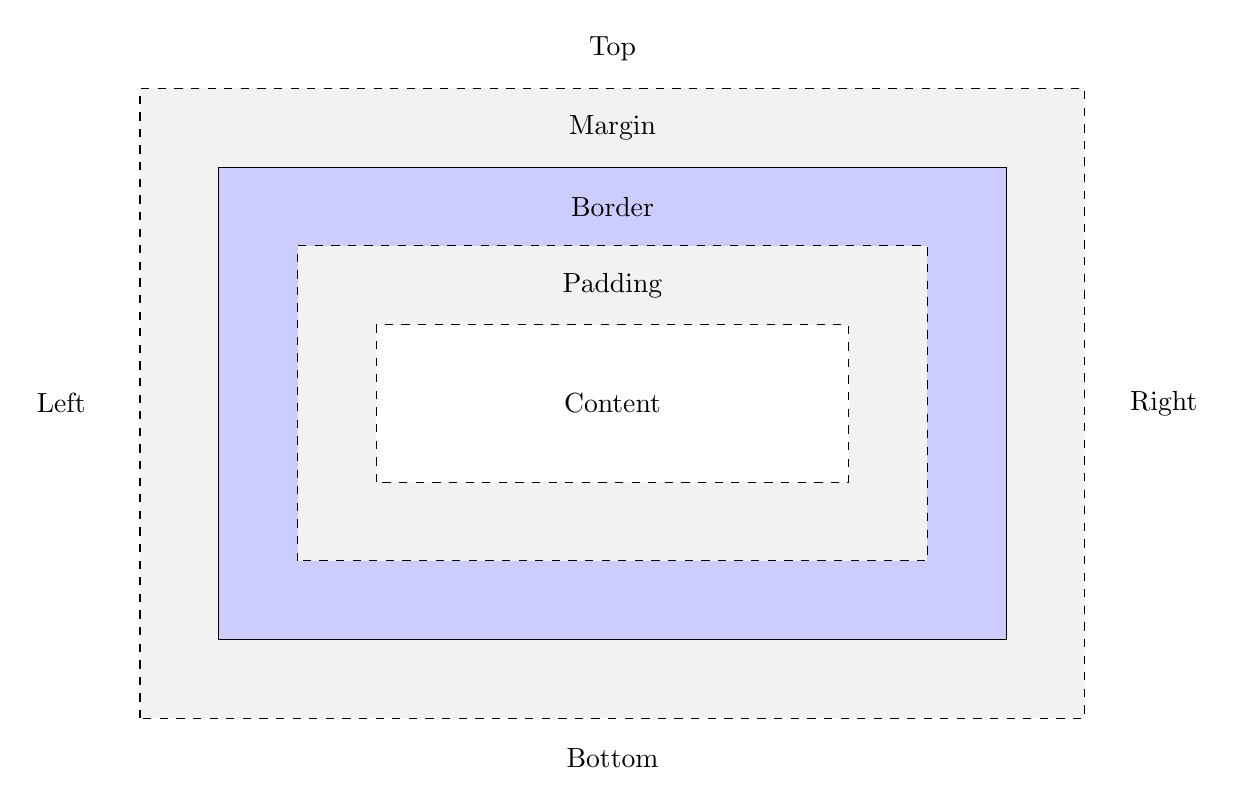
\begin{tikzpicture}
    \draw[dashed,fill=gray!10] (0, 0) rectangle (12, 8);
    \draw[fill=blue!20] (1, 1) rectangle (11, 7);
    \draw[dashed,fill=gray!10] (2, 2) rectangle (10, 6);
    \draw[dashed,fill=white] (3, 3) rectangle (9, 5);

    \node at (6, 4) {Content};
    \node at (6, 5.5) {Padding};
    \node at (6, 6.5) {Border};
    \node at (6, 7.5) {Margin};

    \node at (6, 8.5) {Top};
    \node at (13, 4) {Right};
    \node at (-1, 4) {Left};
    \node at (6, -0.5) {Bottom};
  \end{tikzpicture}
  \caption{The Box Model}
\end{figure}

\begin{enumerate}
  \item \textbf{Content} - The content area is where the text and images
        of the element are displayed. The content area is defined by the width
        and height of the element.

  \item \textbf{Padding} - The padding area is the space between the
        content area and the border of the element. Padding is used to create
        space around the content.

  \item \textbf{Border} - The border area is the line that surrounds the
        padding and content of the element. The border is used to define the
        visual appearance of the element.

  \item \textbf{Margin} - The margin area is the space outside the border
        of the element. The margin is used to create space between elements.
\end{enumerate}

\subsubsection{Units}

In CSS, there are different units that can be used to define the size of
elements. Some of the common units include:

\begin{enumerate}
  \item \textbf{Pixels (px)} - Pixels are a fixed unit of measurement
        that is used to define the size of elements in terms of screen pixels.
        Pixels are an absolute unit and do not change based on the screen size.

  \item \textbf{Percent (\%)} - Percentages are a relative unit of
        measurement that is used to define the size of elements as a percentage
        of the parent element. Percentages are relative to the parent element
        and change based on the size of the parent element.

  \item \textbf{Em (em)} - Em is a relative unit of measurement that is
        used to define the size of elements relative to the font size of the
        parent element. Em is relative to the font size of the parent element
        and changes based on the font size of the parent element.

  \item \textbf{Rem (rem)} - Rem is a relative unit of measurement that
        is used to define the size of elements relative to the font size of the
        root element (html). Rem is relative to the font size of the root element
        and does not change based on the font size of the parent element.

  \item \textbf{Viewport Width (vw)} - Viewport width is a relative unit
        of measurement that is used to define the size of elements relative to
        the width of the viewport. Viewport width is relative to the width of
        the viewport and changes based on the size of the viewport.

  \item \textbf{Viewport Height (vh)} - Viewport height is a relative unit
        of measurement that is used to define the size of elements relative to
        the height of the viewport. Viewport height is relative to the height of
        the viewport and changes based on the size of the viewport.
\end{enumerate}

\subsection{Properties}

\subsubsection{Colors}

In CSS, colors can be specified using different formats, such as color names,
hexadecimal values, RGB values, and HSL values.

\paragraph{Font Color}

The \textbf{color} property is used to set the color of the text.

\begin{lstlisting}[language=HTML, caption={Font Color HTML}, label={lst:font-color-html}]
<p>This is a paragraph.</p>
\end{lstlisting}

\begin{lstlisting}[language=HTML, caption={Font Color CSS}, label={lst:font-color-css}]
p {
  color: red;
}
\end{lstlisting}

Code \ref{lst:font-color-html} and \ref{lst:font-color-css} show an example of
the \textbf{color} property. In this example, the color of the text in the
\textbf{<p>} element is set to red.

\paragraph{Background Color}

The \textbf{background-color} property is used to set the background color of
an element.

\begin{lstlisting}[language=HTML, caption={Background Color HTML}, label={lst:background-color-html}]
<div>
  <h1>Welcome to my website</h1>
</div>
\end{lstlisting}

\begin{lstlisting}[language=HTML, caption={Background Color CSS}, label={lst:background-color-css}]
div {
  background-color: lightblue;
}
\end{lstlisting}

Code \ref{lst:background-color-html} and \ref{lst:background-color-css} show an
example of the \textbf{background-color} property. In this example, the
background color of the \textbf{<div>} element is set to light blue.

\paragraph{Border Color}

The \textbf{border-color} property is used to set the color of the border of an
element.

\begin{lstlisting}[language=HTML, caption={Border Color HTML}, label={lst:border-color-html}]
<div>
  <h1>Welcome to my website</h1>
</div>
\end{lstlisting}

\begin{lstlisting}[language=HTML, caption={Border Color CSS}, label={lst:border-color-css}]
div {
  border: 1px solid black;
}
\end{lstlisting}

Code \ref{lst:border-color-html} and \ref{lst:border-color-css} show an example
of the \textbf{border-color} property. In this example, the border color of the
\textbf{<div>} element is set to black.

\paragraph{Color Names}

CSS provides a set of predefined color names that can be used to specify
colors. Some of the common color names include:

\begin{itemize}
  \item \textbf{Red} - red
  \item \textbf{Green} - green
  \item \textbf{Blue} - blue
  \item \textbf{Black} - black
  \item \textbf{White} - white
  \item \textbf{Yellow} - yellow
  \item \textbf{Purple} - purple
  \item \textbf{Orange} - orange
  \item \textbf{Gray} - gray
  \item \textbf{Brown} - brown
  \item \textbf{Pink} - pink
  \item \href{https://www.w3schools.com/tags/ref_colornames.asp}{More...}
\end{itemize}

\begin{lstlisting}[language=HTML, caption={Color Names HTML}, label={lst:color-names-html}]
<p>This is a paragraph.</p>
\end{lstlisting}

\begin{lstlisting}[language=HTML, caption={Color Names CSS}, label={lst:color-names-css}]
p {
  color: blue;
  background-color: yellow;
  border-color: red;
}
\end{lstlisting}

Code \ref{lst:color-names-html} and \ref{lst:color-names-css} show an example
of using color names to set the color of the text, background, and border of
the \textbf{<p>} element to blue, yellow, and red, respectively.

\paragraph{Hexadecimal Colors}

\textbf{Hexadecimal colors} are represented using a six-digit code that
defines the amount of red, green, and blue as well as the transparency
of the color. The code starts with a hash (\#) followed by the six-digit
hexadecimal code - \textbf{\#RRGGBB}. Eight digits can be used to include the
alpha channel - \textbf{\#RRGGBBAA}.

\begin{lstlisting}[language=HTML, caption={Hexadecimal Colors HTML}, label={lst:hex-colors-html}]
<div>
  <h1>Welcome to my website</h1>
</div>
\end{lstlisting}

\begin{lstlisting}[language=HTML, caption={Hexadecimal Colors CSS}, label={lst:hex-colors-css}]
div {
  color: #ff0000; /* Red */
  background-color: #00ff00; /* Green */
  border-color: #0000ff; /* Blue */
}
\end{lstlisting}

Code \ref{lst:hex-colors-html} and \ref{lst:hex-colors-css} show an example of
using hexadecimal colors to set the color of the text, background, and border
of the \textbf{<div>} element to red, green, and blue, respectively.

\paragraph{RGB or RGBA Colors}

\textbf{RGB colors} are represented using the RGB color model, which defines
the amount of red, green, and blue in the color. The RGB color is defined
using the \textbf{rgb()} function with three values for red, green, and blue.
The \textbf{RGBA colors} include an additional value for the alpha channel
(transparency) and are defined using the \textbf{rgba()} function.

\begin{lstlisting}[language=HTML, caption={RGB Colors HTML}, label={lst:rgb-colors-html}]
<p>This is a paragraph.</p>
\end{lstlisting}

\begin{lstlisting}[language=HTML, caption={RGB Colors CSS}, label={lst:rgb-colors-css}]
p {
  color: rgb(255, 0, 0); /* Red */
  background-color: rgba(0, 255, 0, 0.5); /* Green with 50% opacity */
}
\end{lstlisting}

Code \ref{lst:rgb-colors-html} and \ref{lst:rgb-colors-css} show an example of
using RGB and RGBA colors to set the color of the text in the \textbf{<p>}
element to red and the background color to green with 50\% opacity.

\paragraph{HSL or HSLA Colors}

\textbf{HSL colors} are represented using the HSL color model, which defines
the hue, saturation, and lightness of the color. The HSL color is defined
using the \textbf{hsl()} function with three values for hue, saturation, and
lightness. The \textbf{HSLA colors} include an additional value for the alpha
channel (transparency) and are defined using the \textbf{hsla()} function.

\begin{lstlisting}[language=HTML, caption={HSL Colors HTML}, label={lst:hsl-colors-html}]
<p>This is a paragraph.</p>
\end{lstlisting}

\begin{lstlisting}[language=HTML, caption={HSL Colors CSS}, label={lst:hsl-colors-css}]
p {
  color: hsl(0, 100%, 50%); /* Red */
  background-color: hsla(120, 100%, 50%, 0.5); /* Green with 50% opacity */
}
\end{lstlisting}

Code \ref{lst:hsl-colors-html} and \ref{lst:hsl-colors-css} show an example of
using HSL and HSLA colors to set the color of the text in the \textbf{<p>}
element to red and the background color to green with 50\% opacity.

\paragraph{Gradients}

\textbf{Gradients} are used to create a smooth transition between two or more
colors. Gradients can be linear or radial and can be defined using the
\textbf{linear-gradient()} or \textbf{radial-gradient()} function.

\begin{lstlisting}[language=HTML, caption={Gradients HTML}, label={lst:gradients-html}]
<div>
  <h1>Welcome to my website</h1>
</div>
\end{lstlisting}

\begin{lstlisting}[language=HTML, caption={Gradients CSS}, label={lst:gradients-css}]
div {
  padding: 20px;
  background-image: linear-gradient(to right, red, blue);
}
\end{lstlisting}

Code \ref{lst:gradients-html} and \ref{lst:gradients-css} show an example of
using gradients to set the background color of the \textbf{<div>} element to a
linear gradient from red to blue.

\paragraph{CSS Background Image}

The \textbf{background-image} property is used to specify the background image
for an element. The value can be a URL to an image file or a gradient.

\begin{lstlisting}[language=HTML, caption={Background Image}, label={lst:background-image}]
div {
  padding: 20px;
  background-image: url('https://picsum.photos/200');
}
\end{lstlisting}

Code \ref{lst:background-image} shows an example of using the
\textbf{background-image} property to set the background image for the
\textbf{<div>} element to an image from the URL.

\paragraph{CSS Background Size}

The \textbf{background-size} property is used to specify the size of the
background image. It can be set to a specific size, such as \textbf{cover} or
\textbf{contain}, or to a percentage of the element's width and height.

\begin{lstlisting}[language=HTML, caption={Background Size}, label={lst:background-size}]
div {
  padding: 20px;
  background-image: url('https://picsum.photos/200');
  background-size: cover;
}
\end{lstlisting}

Code \ref{lst:background-size} shows an example of using the
\textbf{background-size} property to set the size of the background image for
the \textbf{<div>} element to cover the entire element.

\subsubsection{Box}

\paragraph{Margin}

The \textbf{margin} property is used to set the margin of an element. The
margin is the space outside the border of the element and is used to create
space between elements.

\begin{lstlisting}[language=HTML, caption={Margin HTML}, label={lst:margin-html}]
<div class="container">
  <div class="item">Item 1</div>
  <div class="item">Item 2</div>
  <div class="item">Item 3</div>
</div>
\end{lstlisting}

\begin{lstlisting}[language=HTML, caption={Margin CSS}, label={lst:margin-css}]
.container {
  display: flex;
  flex-direction: column;
}

.item {
  margin: 10px;
  width: 100px;
  height: 100px;
  background-color: lightblue;
}
\end{lstlisting}

Code \ref{lst:margin-html} and \ref{lst:margin-css} show an example of the
\textbf{margin} property. In this example, the margin of the \textbf{<div>}
element is set to 10 pixels, creating space around the element.

\paragraph{Padding}

The \textbf{padding} property is used to set the padding of an element. The
padding is the space between the content area and the border of the element and
is used to create space around the content.

\begin{lstlisting}[language=HTML, caption={Padding HTML}, label={lst:padding-html}]
<div class="container">
  <div class="item">Item 1</div>
  <div class="item">Item 2</div>
  <div class="item">Item 3</div>
</div>
\end{lstlisting}

\begin{lstlisting}[language=HTML, caption={Padding CSS}, label={lst:padding-css}]
.container {
  display: flex;
  flex-direction: column;
}

.item {
  padding: 10px;
  width: 100px;
  height: 100px;
  background-color: lightblue;
}
\end{lstlisting}

Code \ref{lst:padding-html} and \ref{lst:padding-css} show an example of the
\textbf{padding} property. In this example, the padding of the \textbf{<div>}
element is set to 10 pixels, creating space around the content.

\paragraph{Border}

The \textbf{border} property is used to set the border of an element. The
border is the line that surrounds the padding and content of the element and is
used to define the visual appearance of the element.

\begin{lstlisting}[language=HTML, caption={Border HTML}, label={lst:border-html}]
<div class="container">
  <div class="item">Item 1</div>
  <div class="item">Item 2</div>
  <div class="item">Item 3</div>
</div>
\end{lstlisting}

\begin{lstlisting}[language=HTML, caption={Border CSS}, label={lst:border-css}]
.container {
  display: flex;
  flex-direction: column;
}

.item {
  padding: 4px;m
  margin: 4px;
  border: 1px solid black;
  width: 100px;
  height: 100px;
  background-color: lightblue;
}
\end{lstlisting}

Code \ref{lst:border-html} and \ref{lst:border-css} show an example of the
\textbf{border} property. In this example, the border of the \textbf{<div>}
element is set to 1 pixel solid black, creating a border around the element.

\paragraph{Space Between}

The \textbf{space-between} property is used to set the space between elements
in a flex container. It distributes the extra space between elements in the
container.

\begin{lstlisting}[language=HTML, caption={Space Between HTML}, label={lst:space-between HTML}]
<div class="container">
  <div class="item">Item 1</div>
  <div class="item">Item 2</div>
  <div class="item">Item 3</div>
</div>
\end{lstlisting}

\begin{lstlisting}[language=HTML, caption={Space Between CSS}, label={lst:space-between CSS}]
.container {
  display: flex;
  justify-content: space-between;
}

.item {
  width: 100px;
  height: 100px;
  background-color: lightblue;
}
\end{lstlisting}

Code \ref{lst:space-between HTML} and \ref{lst:space-between CSS} show an
example of the \textbf{space-between} property. In this example, the
\textbf{justify-content} property is set to \textbf{space-between} to
distribute the extra space between the elements in the \textbf{<div>}
container.

\paragraph{Width and Height}

The \textbf{width} and \textbf{height} properties are used to set the width and
height of an element. The width and height can be set to a specific size, such
as pixels or percentages, or to \textbf{auto} to automatically adjust to the
content.

\begin{lstlisting}[language=HTML, caption={Width and Height HTML}, label={lst:width-height-html}]
<div class="container">
  <div class="item1">Item 1</div>
  <div class="item2">Item 2</div>
  <div class="item3">Item 3</div>
</div>
\end{lstlisting}

\begin{lstlisting}[language=HTML, caption={Width and Height CSS}, label={lst:width-height-css}]
.container {
  display: flex;
  flex-direction: column;
}

.item {
  background-color: lightblue;
}

.item1 {
  width: 100px;
  height: 100px;
}

.item2 {
  width: 50%;
  height: 50%;
}

.item3 {
  width: auto;
  height: auto;
}
\end{lstlisting}

Code \ref{lst:width-height-html} and \ref{lst:width-height-css} show an example
of the \textbf{width} and \textbf{height} properties. In this example, the
width and height of the \textbf{<div>} elements are set to 100 pixels, 50\%,
and auto, creating different sizes for the elements.

\paragraph{Radius}

The \textbf{border-radius} property is used to set the radius of the corners of
an element. The radius can be set to a specific size, such as pixels or
percentages, to create rounded corners.

\begin{lstlisting}[language=HTML, caption={Radius HTML}, label={lst:radius-html}]
<div class="container">
  <div class="item1">Item 1</div>
  <div class="item2">Item 2</div>
  <div class="item3">Item 3</div>
</div>
\end{lstlisting}

\begin{lstlisting}[language=HTML, caption={Radius CSS}, label={lst:radius-css}]
.container {
  display: flex;
  flex-direction: column;
}

.item {
  width: 100px;
  height: 100px;
  background-color: lightblue;
}

.item1 {
  border-radius: 50%;
}

.item2 {
  border-radius: 10px;
}

.item3 {
  border-radius: 20%;
}
\end{lstlisting}

Code \ref{lst:radius-html} and \ref{lst:radius-css} show an example of the
\textbf{border-radius} property. In this example, the radius of the corners of
the \textbf{<div>} element is set to 50\%, 10 pixels, and 20\%, creating
different levels of rounded corners.

\paragraph{Box Shadow}

The \textbf{box-shadow} property is used to add a shadow effect to an element.
The shadow can be set to a specific size, color, and blur radius to create
different shadow effects.

\begin{lstlisting}[language=HTML, caption={Box Shadow HTML}, label={lst:box-shadow-html}]
<div class="container">
  <div class="item1">Item 1</div>
  <div class="item2">Item 2</div>
  <div class="item3">Item 3</div>
</div>
\end{lstlisting}

\begin{lstlisting}[language=HTML, caption={Box Shadow CSS}, label={lst:box-shadow-css}]
.container {
  display: flex;
  flex-direction: column;
}

.item {
  width: 100px;
  height: 100px;
  background-color: lightblue;
}

.item1 {
  box-shadow: 5px 5px 5px black;
}

.item2 {
  box-shadow: 10px 10px 10px red;
}

.item3 {
  box-shadow: 0 0 10px blue;
}
\end{lstlisting}

Code \ref{lst:box-shadow-html} and \ref{lst:box-shadow-css} show an example of
the \textbf{box-shadow} property. In this example, the shadow effect of the
\textbf{<div>} element is set to 5 pixels black, 10 pixels red, and 10 pixels
blue, creating different shadow effects.

\paragraph{Opacity}

The \textbf{opacity} property is used to set the opacity of an element. The
opacity can be set to a value between 0 and 1, where 0 is fully transparent and
1 is fully opaque.

\begin{lstlisting}[language=HTML, caption={Opacity HTML}, label={lst:opacity-html}]
<div class="container">
  <div class="item1">Item 1</div>
  <div class="item2">Item 2</div>
  <div class="item3">Item 3</div>
</div>
\end{lstlisting}

\begin{lstlisting}[language=HTML, caption={Opacity CSS}, label={lst:opacity-css}]
.container {
  display: flex;
  flex-direction: column;
}

.item {
  width: 100px;
  height: 100px;
  background-color: lightblue;
}

.item1 {
  opacity: 0.5;
}

.item2 {
  opacity: 0.7;
}

.item3 {
  opacity: 0.9;
}
\end{lstlisting}

Code \ref{lst:opacity-html} and \ref{lst:opacity-css} show an example of the
\textbf{opacity} property. In this example, the opacity of the \textbf{<div>}
element is set to 0.5, 0.7, and 0.9, creating different levels of transparency.
The higher the value, the more opaque the element.

\subsubsection{Text}

\paragraph{Text Align}

\paragraph{Text Decoration}

\paragraph{Text Transform}

\paragraph{Line Height}

\paragraph{Font Family}

\paragraph{Font Size}

\paragraph{Font Weight}

\paragraph{Font Style}

\subsubsection{Layout}

\paragraph{Display}

\paragraph{Flexbox}

\paragraph{Grid}

\subsubsection{Positioning}

\paragraph{Static}

\paragraph{Relative}

\paragraph{Absolute}

\paragraph{Fixed}

\paragraph{Sticky}

\subsubsection{Transforms}

\paragraph{Scale}

\paragraph{Rotate}

\paragraph{Skew}

\paragraph{Translate}

\paragraph{Origin}

\subsubsection{Interactivity}

\paragraph{Hover}

\paragraph{Focus}

\paragraph{Active}

\paragraph{Transition}

\paragraph{Animation}

\subsubsection{Filters}

\paragraph{Blur}

\paragraph{Brightness}

\paragraph{Contrast}

\paragraph{Drop Shadow}

\paragraph{Grayscale}

\paragraph{Hue Rotate}

\paragraph{Invert}

\paragraph{Opacity}

\paragraph{Saturate}

\paragraph{Sepia}

\subsubsection{Responsive Design}

\paragraph{Media Queries}

\paragraph{Viewport}

\paragraph{Responsive Images}

\subsection{Frameworks}

\subsubsection{Bootstrap}

\subsubsection{Tailwind CSS}

\subsection{More about CSS}

You can find more information about CSS properties from the following sources:

\begin{itemize}
  \item \href{https://developer.mozilla.org/en-US/docs/Web/CSS/Reference}{MDN Web Docs CSS Reference}
  \item \href{https://www.w3schools.com/cssref/default.asp}{W3Schools CSS Reference}
  \item \href{https://www.toptal.com/css/css-cheat-sheet}{Toptal CSS Cheat Sheet}
\end{itemize}

\chapter{Version Control}

\chapter{NextJS}

\chapter{Mobile Applications Development}

\chapter{Cloud Computing}

\chapter{Artificial Intelligence}

\chapter{Internet of Things and Augmented Reality}

\begin{enumerate}[label={\textbf{\Alph*.}}]
  \item \textbf{Books}
        \begin{itemize}
          \item
        \end{itemize}
  \item \textbf{Other Sources}
        \begin{itemize}
          \item
        \end{itemize}
\end{enumerate}

\end{document}
